\begin{enumerate}
    \item Vào giờ ra chơi ở một trường nọ, có bốn bạn đang băng qua sân trường rộng lớn cùng lúc, khi bắt đầu chuyển động, \textit{vận tốc các bạn không đổi và khác nhau}, phương các vận tốc \textit{không song song nhau và không có quá hai phương chuyển động đồng quy tại một điểm}. Biết \textit{5 và chỉ 5 trên 6 trường hợp} các bạn có thể gặp nhau đã xảy ra. Cho rằng vận tốc các bạn không đổi suốt quá trình chuyển động và mỗi lần gặp nhau không ảnh hưởng gì tới sự chuyển động của các bạn. \textbf{Trường hợp gặp nhau thứ 6 có xảy ra không?}  
    %Nguồn: \textit{200 Puzzling Physics Problems}
\begin{figure}[ht]
    \centering
    \scalebox{1.1}{
    \tikzset{every picture/.style={line width=0.75pt}} %set default line width to 0.75pt        
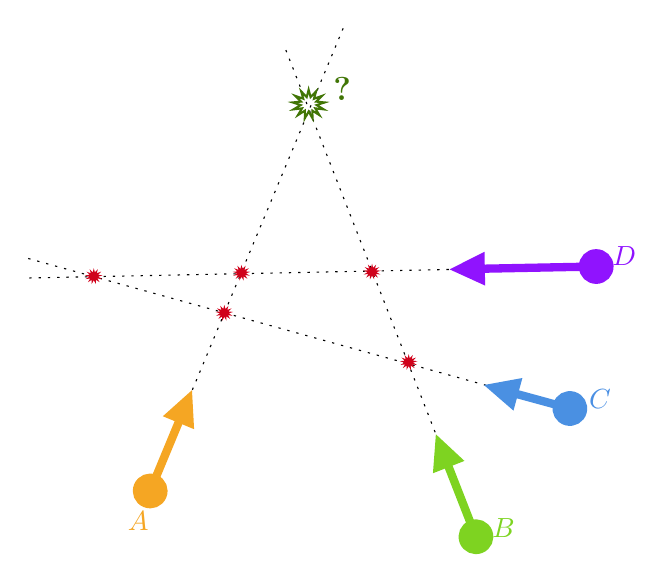
\begin{tikzpicture}[x=0.75pt,y=0.75pt,yscale=-1,xscale=1]
%uncomment if require: \path (0,7622); %set diagram left start at 0, and has height of 7622

%Straight Lines [id:da4257880873279283] 
\draw  [dash pattern={on 0.84pt off 2.51pt}]  (251.22,4004.97) -- (158.26,4227.86) ;
\draw [shift={(158.26,4227.86)}, rotate = 112.64] [color={rgb, 255:red, 0; green, 0; blue, 0 }  ][fill={rgb, 255:red, 0; green, 0; blue, 0 }  ][line width=0.75]      (0, 0) circle [x radius= 3.35, y radius= 3.35]   ;
%Straight Lines [id:da9952714607108861] 
\draw  [dash pattern={on 0.84pt off 2.51pt}]  (223.63,4015.45) -- (315.21,4249.92) ;
\draw [shift={(315.21,4249.92)}, rotate = 68.66] [color={rgb, 255:red, 0; green, 0; blue, 0 }  ][fill={rgb, 255:red, 0; green, 0; blue, 0 }  ][line width=0.75]      (0, 0) circle [x radius= 3.35, y radius= 3.35]   ;
%Straight Lines [id:da9393707554836688] 
\draw  [dash pattern={on 0.84pt off 2.51pt}]  (99.5,4115.86) -- (360.45,4188.13) ;
\draw [shift={(360.45,4188.13)}, rotate = 15.48] [color={rgb, 255:red, 0; green, 0; blue, 0 }  ][fill={rgb, 255:red, 0; green, 0; blue, 0 }  ][line width=0.75]      (0, 0) circle [x radius= 3.35, y radius= 3.35]   ;
%Straight Lines [id:da4242707810533324] 
\draw  [dash pattern={on 0.84pt off 2.51pt}]  (100.05,4125.24) -- (373.14,4119.72) ;
\draw [shift={(373.14,4119.72)}, rotate = 358.84] [color={rgb, 255:red, 0; green, 0; blue, 0 }  ][fill={rgb, 255:red, 0; green, 0; blue, 0 }  ][line width=0.75]      (0, 0) circle [x radius= 3.35, y radius= 3.35]   ;
%Straight Lines [id:da5822274503273119] 
\draw [color={rgb, 255:red, 126; green, 211; blue, 33 }  ,draw opacity=1 ][line width=3]    (315.21,4249.92) -- (298.09,4206.13) ;
\draw [shift={(295.9,4200.55)}, rotate = 68.64] [fill={rgb, 255:red, 126; green, 211; blue, 33 }  ,fill opacity=1 ][line width=0.08]  [draw opacity=0] (16.97,-8.15) -- (0,0) -- (16.97,8.15) -- cycle    ;
\draw [shift={(315.21,4249.92)}, rotate = 248.64] [color={rgb, 255:red, 126; green, 211; blue, 33 }  ,draw opacity=1 ][fill={rgb, 255:red, 126; green, 211; blue, 33 }  ,fill opacity=1 ][line width=3]      (0, 0) circle [x radius= 6.37, y radius= 6.37]   ;
%Straight Lines [id:da051074197187332526] 
\draw [color={rgb, 255:red, 245; green, 166; blue, 35 }  ,draw opacity=1 ][line width=3]    (158.26,4227.86) -- (176.09,4184.85) ;
\draw [shift={(178.39,4179.31)}, rotate = 112.53] [fill={rgb, 255:red, 245; green, 166; blue, 35 }  ,fill opacity=1 ][line width=0.08]  [draw opacity=0] (16.97,-8.15) -- (0,0) -- (16.97,8.15) -- cycle    ;
\draw [shift={(158.26,4227.86)}, rotate = 292.53] [color={rgb, 255:red, 245; green, 166; blue, 35 }  ,draw opacity=1 ][fill={rgb, 255:red, 245; green, 166; blue, 35 }  ,fill opacity=1 ][line width=3]      (0, 0) circle [x radius= 6.37, y radius= 6.37]   ;
%Straight Lines [id:da17569860173881802] 
\draw [color={rgb, 255:red, 74; green, 144; blue, 226 }  ,draw opacity=1 ][line width=3]    (360.45,4188.13) -- (324.86,4178.41) ;
\draw [shift={(319.07,4176.82)}, rotate = 15.29] [fill={rgb, 255:red, 74; green, 144; blue, 226 }  ,fill opacity=1 ][line width=0.08]  [draw opacity=0] (16.97,-8.15) -- (0,0) -- (16.97,8.15) -- cycle    ;
\draw [shift={(360.45,4188.13)}, rotate = 195.29] [color={rgb, 255:red, 74; green, 144; blue, 226 }  ,draw opacity=1 ][fill={rgb, 255:red, 74; green, 144; blue, 226 }  ,fill opacity=1 ][line width=3]      (0, 0) circle [x radius= 6.37, y radius= 6.37]   ;
%Straight Lines [id:da02986144608238317] 
\draw [color={rgb, 255:red, 144; green, 19; blue, 254 }  ,draw opacity=1 ][line width=3]    (373.14,4119.72) -- (308.52,4120.98) ;
\draw [shift={(302.52,4121.1)}, rotate = 358.88] [fill={rgb, 255:red, 144; green, 19; blue, 254 }  ,fill opacity=1 ][line width=0.08]  [draw opacity=0] (16.97,-8.15) -- (0,0) -- (16.97,8.15) -- cycle    ;
\draw [shift={(373.14,4119.72)}, rotate = 178.88] [color={rgb, 255:red, 144; green, 19; blue, 254 }  ,draw opacity=1 ][fill={rgb, 255:red, 144; green, 19; blue, 254 }  ,fill opacity=1 ][line width=3]      (0, 0) circle [x radius= 6.37, y radius= 6.37]   ;
%Shape: Star [id:dp4652455317009081] 
\draw  [draw opacity=0][fill={rgb, 255:red, 208; green, 2; blue, 27 }  ,fill opacity=1 ] (202.25,4118.9) -- (202.76,4120.88) -- (204.24,4119.34) -- (203.67,4121.31) -- (205.77,4120.56) -- (204.25,4122.07) -- (206.5,4122.29) -- (204.38,4122.99) -- (206.25,4124.13) -- (204.01,4123.85) -- (205.09,4125.65) -- (203.25,4124.47) -- (203.28,4126.51) -- (202.25,4124.69) -- (201.23,4126.51) -- (201.26,4124.47) -- (199.42,4125.65) -- (200.49,4123.85) -- (198.26,4124.13) -- (200.13,4122.99) -- (198.01,4122.29) -- (200.25,4122.07) -- (198.73,4120.56) -- (200.84,4121.31) -- (200.27,4119.34) -- (201.74,4120.88) -- cycle ;
%Shape: Star [id:dp17943360623521842] 
\draw  [draw opacity=0][fill={rgb, 255:red, 208; green, 2; blue, 27 }  ,fill opacity=1 ] (131.08,4120.55) -- (131.6,4122.54) -- (133.07,4120.99) -- (132.5,4122.97) -- (134.6,4122.22) -- (133.08,4123.73) -- (135.33,4123.95) -- (133.21,4124.64) -- (135.08,4125.78) -- (132.84,4125.51) -- (133.92,4127.3) -- (132.08,4126.12) -- (132.11,4128.16) -- (131.08,4126.34) -- (130.06,4128.16) -- (130.09,4126.12) -- (128.25,4127.3) -- (129.33,4125.51) -- (127.09,4125.78) -- (128.96,4124.64) -- (126.84,4123.95) -- (129.09,4123.73) -- (127.57,4122.22) -- (129.67,4122.97) -- (129.1,4120.99) -- (130.57,4122.54) -- cycle ;
%Shape: Star [id:dp03789410132743454] 
\draw  [draw opacity=0][fill={rgb, 255:red, 208; green, 2; blue, 27 }  ,fill opacity=1 ] (265.15,4118.34) -- (265.66,4120.33) -- (267.13,4118.79) -- (266.56,4120.76) -- (268.67,4120.01) -- (267.15,4121.52) -- (269.39,4121.74) -- (267.27,4122.44) -- (269.14,4123.57) -- (266.91,4123.3) -- (267.98,4125.1) -- (266.14,4123.92) -- (266.17,4125.96) -- (265.15,4124.14) -- (264.12,4125.96) -- (264.15,4123.92) -- (262.31,4125.1) -- (263.39,4123.3) -- (261.15,4123.57) -- (263.02,4122.44) -- (260.9,4121.74) -- (263.15,4121.52) -- (261.63,4120.01) -- (263.73,4120.76) -- (263.16,4118.79) -- (264.64,4120.33) -- cycle ;
%Shape: Star [id:dp6092374284959783] 
\draw  [draw opacity=0][fill={rgb, 255:red, 208; green, 2; blue, 27 }  ,fill opacity=1 ] (193.98,4138.2) -- (194.49,4140.19) -- (195.96,4138.65) -- (195.4,4140.62) -- (197.5,4139.87) -- (195.98,4141.38) -- (198.22,4141.6) -- (196.1,4142.3) -- (197.98,4143.44) -- (195.74,4143.16) -- (196.81,4144.96) -- (194.97,4143.78) -- (195,4145.82) -- (193.98,4144) -- (192.95,4145.82) -- (192.98,4143.78) -- (191.14,4144.96) -- (192.22,4143.16) -- (189.98,4143.44) -- (191.86,4142.3) -- (189.73,4141.6) -- (191.98,4141.38) -- (190.46,4139.87) -- (192.56,4140.62) -- (191.99,4138.65) -- (193.47,4140.19) -- cycle ;
%Shape: Star [id:dp9525934681135235] 
\draw  [draw opacity=0][fill={rgb, 255:red, 208; green, 2; blue, 27 }  ,fill opacity=1 ] (282.8,4161.93) -- (283.31,4163.91) -- (284.79,4162.37) -- (284.22,4164.34) -- (286.32,4163.6) -- (284.8,4165.1) -- (287.05,4165.32) -- (284.92,4166.02) -- (286.8,4167.16) -- (284.56,4166.89) -- (285.64,4168.68) -- (283.79,4167.5) -- (283.82,4169.54) -- (282.8,4167.72) -- (281.78,4169.54) -- (281.81,4167.5) -- (279.97,4168.68) -- (281.04,4166.89) -- (278.8,4167.16) -- (280.68,4166.02) -- (278.56,4165.32) -- (280.8,4165.1) -- (279.28,4163.6) -- (281.38,4164.34) -- (280.81,4162.37) -- (282.29,4163.91) -- cycle ;
%Shape: Star [id:dp7689921001871347] 
\draw  [color={rgb, 255:red, 65; green, 117; blue, 5 }  ,draw opacity=1 ][line width=0.75]  (234.6,4034.49) -- (235.53,4038.11) -- (238.22,4035.29) -- (237.18,4038.89) -- (241.01,4037.52) -- (238.24,4040.27) -- (242.33,4040.67) -- (238.47,4041.94) -- (241.88,4044.01) -- (237.81,4043.52) -- (239.77,4046.78) -- (236.41,4044.63) -- (236.47,4048.35) -- (234.6,4045.04) -- (232.74,4048.35) -- (232.79,4044.63) -- (229.44,4046.78) -- (231.4,4043.52) -- (227.32,4044.01) -- (230.74,4041.94) -- (226.87,4040.67) -- (230.96,4040.27) -- (228.19,4037.52) -- (232.02,4038.89) -- (230.98,4035.29) -- (233.67,4038.11) -- cycle ;

% Text Node
\draw (146.27,4236.75) node [anchor=north west][inner sep=0.75pt]   [align=left] {$\displaystyle \textcolor[rgb]{0.96,0.65,0.14}{A}$};
% Text Node
\draw (321.83,4240.13) node [anchor=north west][inner sep=0.75pt]   [align=left] {$\displaystyle \textcolor[rgb]{0.49,0.83,0.13}{B}$};
% Text Node
\draw (368.42,4177.79) node [anchor=north west][inner sep=0.75pt]   [align=left] {$\displaystyle \textcolor[rgb]{0.29,0.56,0.89}{C}$};
% Text Node
\draw (379.64,4108.83) node [anchor=north west][inner sep=0.75pt]   [align=left] {$\displaystyle \textcolor[rgb]{0.56,0.07,1}{D}$};
% Text Node
\draw (245.3,4027.33) node [anchor=north west][inner sep=0.75pt]   [align=left] {\textcolor[rgb]{0.25,0.46,0.02}{\textbf{{\large ?}}}};

\end{tikzpicture}
}
\\
\caption{}
\label{P1.1}
\end{figure}

% \caption{}  %% Lệnh \caption phải để trong môi trường figure nhé
\item Lúc này, khi các bạn thực hiện lại quá trình trên nhưng với giả định rằng khi hai người gặp nhau thì họ "\textit{va chạm đàn hồi}" nhau. \textbf{Hỏi số va chạm lớn nhất mà một người có thể trải nghiệm là bao nhiêu?} Với giả định là các bạn học sinh này có cân nặng như nhau. Bỏ qua ảnh hưởng của kích thước các bạn lên chuyển động và hành động tương tác lẫn nhau.

\begin{figure}[ht]
    \centering
    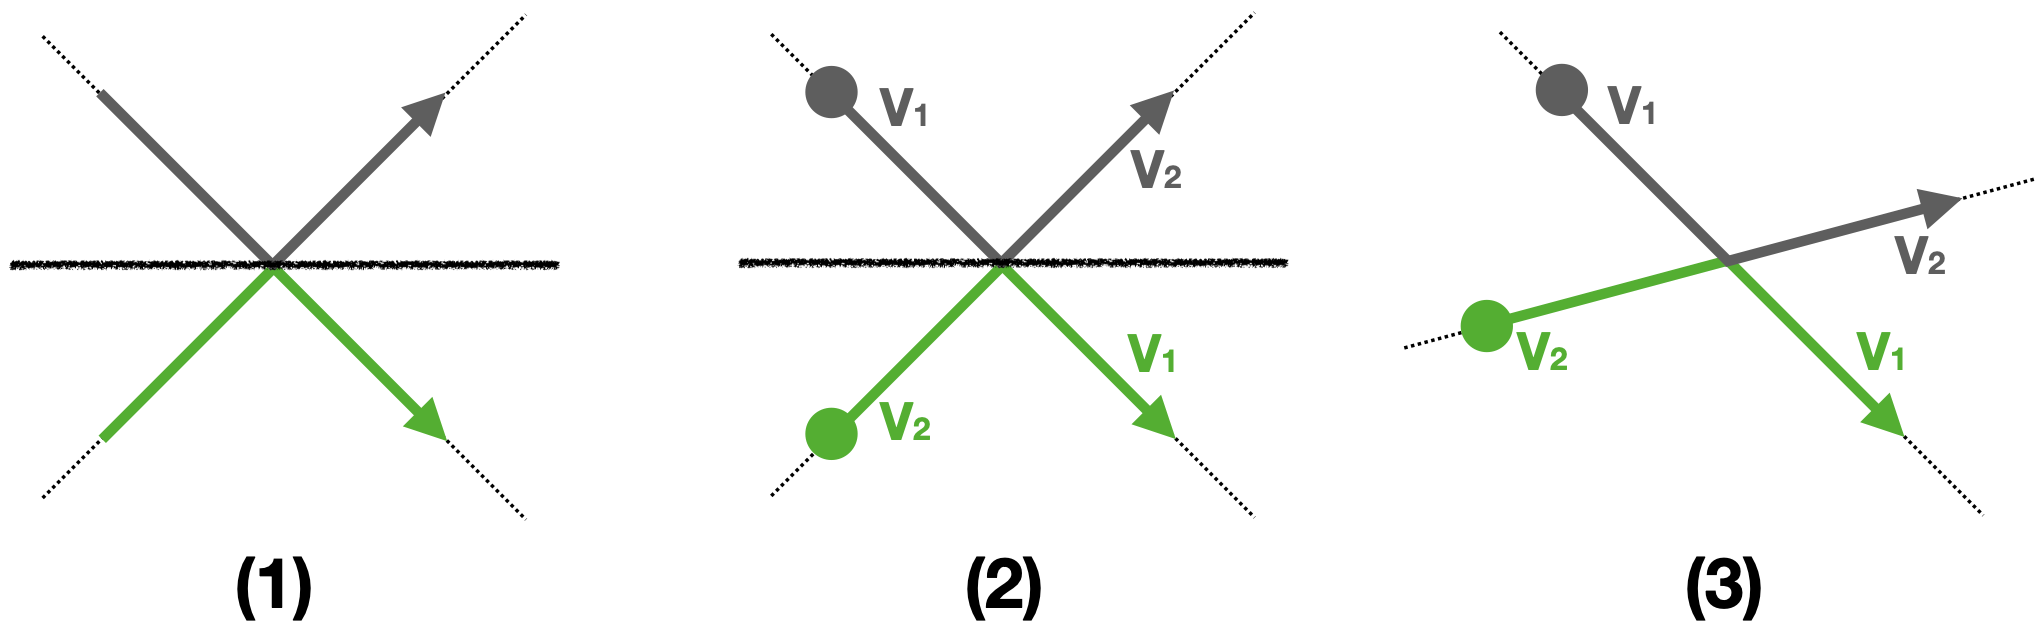
\includegraphics[scale=0.4]{Problem_1/Image/Các trường hợp va chạm đàn hồi.png}
    \caption{}
    \label{P1.2}
\end{figure}


Hành động va chạm đàn hồi của bài có thể dùng hiện tượng phản xạ gương để liên tưởng.

$(1)$ hình ảnh phản xạ gương (tia đen là tia thật, tia xanh là ảnh tia đen qua gương). 

$(2)$ cho hai hạt đi theo quỹ đạo của các tia. 

$(3)$ một va chạm đàn hồi bình thường diễn ra.

Trong các va chạm đàn hồi, các hạt trao đổi \textbf{tốc độ} và \textbf{quỹ đạo} với nhau.
\end{enumerate}
\begin{flushright}
   \normalcolor(Biên soạn bởi wan và Mino)
\end{flushright}